\section{Transformadores}
\label{s.transformer}

\begin{frame}{Transformadores}
	\begin{itemize}
		\justifying
		\item Vaswani et al.~\cite{Vaswani:17} propuseram a primeira arquitetura de Transformadores, do inglês \emph{Transformers};
		\\~\\
		\item São arquiteturas puramente baseadas em mecanismos de Atenção e alternativas às Redes Neurais Recorrentes;	
	\end{itemize}
\end{frame}

\begin{frame}
	\vspace*{0.5cm}
	\begin{figure}[!ht]
		\centering
		\includegraphics[scale=0.45]{figs/transformer.eps}	
		\label{f.transformer}
		\caption{Arquitetura de um Transformador.}
	\end{figure}
\end{frame}

\begin{frame}
	\begin{figure}[!ht]
		\centering
		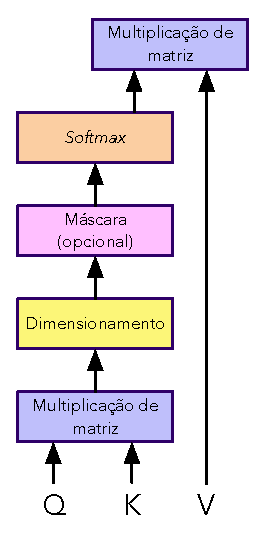
\includegraphics[scale=0.65]{figs/attention.eps}	
		\label{f.attention}
		\caption{Mecanismo de Atenção.}
	\end{figure}
\end{frame}


\begin{frame}
	\begin{figure}[!ht]
		\centering
		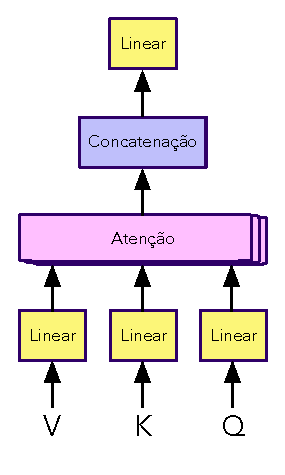
\includegraphics[scale=0.75]{figs/multi_head_attention.eps}	
		\label{f.multi_head_attention}
		\caption{Atenção de Múltiplas Cabeças.}
	\end{figure}
\end{frame}
